% Compiles with IEEEtran (journal) when IEEEtran.cls is available (e.g., Overleaf); otherwise falls back to a
% two-column article layout for local previews. All numbers come from numbers.tex (generated from results/*.json).
\IfFileExists{IEEEtran.cls}{\documentclass[journal]{IEEEtran}\newcommand{\ieeemode}{}}{\documentclass[10pt,twocolumn,letterpaper]{article}\usepackage[margin=0.72in,columnsep=0.22in]{geometry}}
\usepackage[T1]{fontenc}
\usepackage{times}
\usepackage{amsmath,amssymb,amsthm}
\usepackage{graphicx}
\graphicspath{{../figs/}{figs/}}
\usepackage{booktabs}
\usepackage{array}
\newcolumntype{L}[1]{>{\raggedright\arraybackslash}p{#1}}
\usepackage{algorithm}
\usepackage{algpseudocode}
\usepackage{xcolor}
\usepackage[hidelinks]{hyperref}
\usepackage{url}
\usepackage{microtype}
\newtheorem{theorem}{Theorem}
\newtheorem{proposition}[theorem]{Proposition}
\newtheorem{corollary}[theorem]{Corollary}
\newtheorem{assumption}{Assumption}
\renewcommand{\theassumption}{A\arabic{assumption}}
% AUTO-GENERATED by exps/f_numbers.py from results/*.json -- do not edit by hand
\newcommand{\AccAdv}{10}
\newcommand{\AccBasic}{18}
\newcommand{\AccPld}{534}
\newcommand{\AccRdp}{466}
\newcommand{\AfdcFEmax}{6.06}
\newcommand{\AfdcFEmin}{2.80}
\newcommand{\AfilFEmax}{2.31}
\newcommand{\AfilFEmin}{0.00}
\newcommand{\AgridEdge}{8}
\newcommand{\AgridMin}{0.15}
\newcommand{\AirClFdAcc}{0.625}
\newcommand{\AirClFdIso}{5549.7}
\newcommand{\AirClFdIsoPct}{32}
\newcommand{\AirClFdRel}{540}
\newcommand{\AirClFdcAcc}{0.580}
\newcommand{\AirClFdcOut}{1.8}
\newcommand{\AirClFdcPre}{10.4}
\newcommand{\AirClFdcRel}{173}
\newcommand{\AirClFdcTot}{17.3}
\newcommand{\AirClFilAcc}{0.577}
\newcommand{\AirClFilOut}{0.9}
\newcommand{\AirClFilPre}{8.2}
\newcommand{\AirClFilRel}{152}
\newcommand{\AirClFilTot}{15.2}
\newcommand{\AirClLocAcc}{0.589}
\newcommand{\AirClPerAcc}{0.577}
\newcommand{\AirClStaAcc}{0.580}
\newcommand{\AnDetGeq}{5}
\newcommand{\AnDetLower}{3}
\newcommand{\AnLower}{8}
\newcommand{\AnSettings}{8}
\newcommand{\AworstDetC}{0.75}
\newcommand{\AworstDetF}{0.80}
\newcommand{\AworstName}{Elec2, $K=5$}
\newcommand{\BytesAir}{14.2}
\newcommand{\BytesCm}{44.9}
\newcommand{\BytesCov}{75.2}
\newcommand{\BytesElec}{3.2}
\newcommand{\ByzBestAgg}{centered clipping}
\newcommand{\ByzBestWorst}{0.593}
\newcommand{\ByzMeanNone}{0.653}
\newcommand{\ByzMedWorst}{0.538}
\newcommand{\ByzTrimWorst}{0.419}
\newcommand{\ClAccDiffMax}{0.007}
\newcommand{\CmAdjDetFour}{0.775}
\newcommand{\CmAdjDetTwo}{0.935}
\newcommand{\CmAdjFAFour}{0.25}
\newcommand{\CmAdjFATwo}{0.20}
\newcommand{\CmRawDetFour}{0.004}
\newcommand{\CmRawDetTwo}{0.008}
\newcommand{\CmRowsFour}{61,249}
\newcommand{\CmRowsTwo}{53,759}
\newcommand{\CovClFdAcc}{0.778}
\newcommand{\CovClFdIso}{1979.1}
\newcommand{\CovClFdIsoPct}{12}
\newcommand{\CovClFdRel}{540}
\newcommand{\CovClFdcAcc}{0.607}
\newcommand{\CovClFdcOut}{1.2}
\newcommand{\CovClFdcPre}{6.8}
\newcommand{\CovClFdcRel}{99}
\newcommand{\CovClFdcTot}{9.9}
\newcommand{\CovClFilAcc}{0.601}
\newcommand{\CovClFilOut}{0.5}
\newcommand{\CovClFilPre}{5.9}
\newcommand{\CovClFilRel}{84}
\newcommand{\CovClFilTot}{8.4}
\newcommand{\CovClLocAcc}{0.619}
\newcommand{\CovClPerAcc}{0.619}
\newcommand{\CovClStaAcc}{0.453}
\newcommand{\CurveFilDetMax}{1.00}
\newcommand{\CurveFilDetMin}{0.00}
\newcommand{\CurveFilFEmax}{0.00}
\newcommand{\DpCovClip}{0.602}
\newcommand{\DpCovTen}{0.610}
\newcommand{\DpCovTwentyFive}{0.601}
\newcommand{\DpCovZero}{0.639}
\newcommand{\DpElecClip}{0.774}
\newcommand{\DpElecTen}{0.774}
\newcommand{\DpElecZero}{0.769}
\newcommand{\DpEpsTen}{3.5}
\newcommand{\DpLrCov}{20}
\newcommand{\ElecRecFive}{60}
\newcommand{\ElecRecTen}{30}
\newcommand{\EngFour}{249}
\newcommand{\EngTwo}{260}
\newcommand{\FeatAir}{27}
\newcommand{\FeatCov}{54}
\newcommand{\FeatElec}{6}
\newcommand{\FloodOneFE}{0.00}
\newcommand{\GateGainRone}{3.91}
\newcommand{\GateGainRtwenty}{2.26}
\newcommand{\GateHorNoGate}{466}
\newcommand{\HorCont}{74}
\newcommand{\HorFdc}{897}
\newcommand{\HorFdct}{937}
\newcommand{\HorFil}{3,001}
\newcommand{\HorOra}{7,462}
\newcommand{\HorPer}{746}
\newcommand{\HorRatio}{3.3}
\newcommand{\KfourFdcFE}{3.36}
\newcommand{\KfourFilDet}{0.96}
\newcommand{\KtenFilFE}{0.19}
\newcommand{\LegCCmax}{0.050}
\newcommand{\LegCCmin}{0.048}
\newcommand{\LegCorrViol}{0}
\newcommand{\LegN}{45}
\newcommand{\LegViol}{9}
\newcommand{\MagLowFdcDet}{0.80}
\newcommand{\MagLowFilDet}{0.56}
\newcommand{\MagLowFiltTDet}{0.91}
\newcommand{\NonlinFdcFE}{0.76}
\newcommand{\NonlinFilFE}{0.00}
\newcommand{\PfEpsTen}{4.8}
\newcommand{\PfEpsThirty}{1.4}
\newcommand{\PfFEThirty}{3.31}
\newcommand{\PfRel}{104}
\newcommand{\RowsAir}{539,383}
\newcommand{\RowsCov}{581,012}
\newcommand{\RowsElec}{45,312}
\newcommand{\RuntimeHours}{1.9}
\newcommand{\SKeff}{39.4}
\newcommand{\SedFilDelay}{0}
\newcommand{\SedFilDet}{1.000}
\newcommand{\SedFilUCB}{0.26}
\newcommand{\SedRawFA}{140.0}
\newcommand{\SfailHalfFE}{0.40}
\newcommand{\SfailHidFE}{3.33}
\newcommand{\SfailNoiseFE}{4.22}
\newcommand{\SfdcDet}{0.915}
\newcommand{\SfdcFE}{3.41}
\newcommand{\SfdcFEci}{[3.11, 3.71]}
\newcommand{\SfdcHighDet}{0.465}
\newcommand{\SfdcHighFE}{0.59}
\newcommand{\SfdcRawDet}{1.000}
\newcommand{\SfdcW}{170.3}
\newcommand{\SfdctDet}{0.915}
\newcommand{\SfdctFE}{2.97}
\newcommand{\SfilDelay}{3}
\newcommand{\SfilDet}{0.990}
\newcommand{\SfilDetci}{[0.964, 0.997]}
\newcommand{\SfilUCB}{0.026}
\newcommand{\SfiltDet}{1.000}
\newcommand{\SfloodThreeFE}{5.02}
\newcommand{\SfloodTwoFE}{0.38}
\newcommand{\SlocScope}{51.6}
\newcommand{\SlocScopeF}{43.1}
\newcommand{\SlocalW}{256.3}
\newcommand{\SlocfilW}{98.2}
\newcommand{\SpFil}{0.040}
\newcommand{\SpRaw}{0.107}
\newcommand{\SspoofDet}{0.140}
\newcommand{\SsuppThreeDet}{0.570}
\newcommand{\SthetaFdc}{0.45}
\newcommand{\SthetaFil}{0.25}
\newcommand{\SvtActRaw}{0.097}
\newcommand{\SvtCfiveAct}{0.249}
\newcommand{\SvtCfiveFE}{7.17}
\newcommand{\SvtEpsRun}{1.80}
\newcommand{\SvtFilDet}{0.990}
\newcommand{\SvtPosFil}{3.7}
\newcommand{\SvtPosRaw}{9.9}
\newcommand{\TbyzN}{8}
\newcommand{\TbyzViol}{0}
\newcommand{\TccArlHi}{114}
\newcommand{\TccArlLo}{97}
\newcommand{\TdelayHalf}{1}
\newcommand{\TdelayThirty}{4}
\newcommand{\TdetThirty}{0.975}
\newcommand{\TindN}{18}
\newcommand{\TindViol}{0}
\newcommand{\TlongEpochs}{19,980}
\newcommand{\TlongFilFAc}{3}
\newcommand{\TlongFilFAhundred}{0}
\newcommand{\TlongRawArlHi}{8.7}
\newcommand{\TlongRawArlLo}{6.9}
\newcommand{\WcalFdcDeth}{0.945}
\newcommand{\WcalFdcFE}{2.16}
\newcommand{\WcalFdcFEh}{0.71}
\newcommand{\WeqFdcFE}{3.42}

% placeholders for results not yet produced (overridden by numbers.tex when present)
\providecommand{\CovClFdcPre}{\textbf{[TO BE MEASURED]}}
\providecommand{\CovClFilPre}{\textbf{[TO BE MEASURED]}}
\providecommand{\AirClFdcPre}{\textbf{[TO BE MEASURED]}}
\providecommand{\AirClFilPre}{\textbf{[TO BE MEASURED]}}
\providecommand{\CovClFdAcc}{\textbf{[TO BE MEASURED]}}
\providecommand{\AirClFdAcc}{\textbf{[TO BE MEASURED]}}
\providecommand{\CovClFdRel}{\textbf{[TO BE MEASURED]}}
\providecommand{\AirClFdRel}{\textbf{[TO BE MEASURED]}}
\providecommand{\CovClFilRel}{\textbf{[TO BE MEASURED]}}
\providecommand{\AirClFilRel}{\textbf{[TO BE MEASURED]}}
\providecommand{\CovClFdIso}{\textbf{[TO BE MEASURED]}}
\providecommand{\AirClFdIso}{\textbf{[TO BE MEASURED]}}
\providecommand{\CovClFdcAcc}{\textbf{[TO BE MEASURED]}}
\providecommand{\CovClFilAcc}{\textbf{[TO BE MEASURED]}}
\providecommand{\AirClFdcAcc}{\textbf{[TO BE MEASURED]}}
\providecommand{\AirClFilAcc}{\textbf{[TO BE MEASURED]}}
\providecommand{\ByzMeanNone}{\textbf{[TO BE MEASURED]}}
\providecommand{\ByzTrimWorst}{\textbf{[TO BE MEASURED]}}
\providecommand{\ByzMedWorst}{\textbf{[TO BE MEASURED]}}
\providecommand{\ByzBestWorst}{\textbf{[TO BE MEASURED]}}
\providecommand{\ByzBestAgg}{\textbf{[TO BE MEASURED]}}
\providecommand{\DpCovTen}{\textbf{[TO BE MEASURED]}}
\providecommand{\DpCovClip}{\textbf{[TO BE MEASURED]}}
\providecommand{\DpCovZero}{\textbf{[TO BE MEASURED]}}
\providecommand{\DpEpsTen}{\textbf{[TO BE MEASURED]}}
\providecommand{\DpCovTwentyFive}{\textbf{[TO BE MEASURED]}}
\providecommand{\DpElecZero}{\textbf{[TO BE MEASURED]}}
\providecommand{\DpElecTen}{\textbf{[TO BE MEASURED]}}
\makeatletter\newcommand{\inputtable}[1]{\@@input #1 }\makeatother
\newcommand{\safeinput}[1]{\IfFileExists{#1.tex}{\input{#1}}{\multicolumn{8}{c}{\textbf{[TO BE MEASURED]}}\\}}
\newcommand{\safefig}[2]{\IfFileExists{#2}{\includegraphics[width=#1]{#2}}{\fbox{\parbox{#1}{\centering [FIGURE TO BE GENERATED]}}}}
\newcommand{\Keff}{K_{\mathrm{eff}}}
\newcommand{\ARL}{\mathrm{ARL}_0}
% Float placement: allow more floats per page so tables do not end up alone on mostly empty pages.
\renewcommand{\topfraction}{0.9}\renewcommand{\bottomfraction}{0.8}\renewcommand{\textfraction}{0.07}
\renewcommand{\floatpagefraction}{0.85}\renewcommand{\dbltopfraction}{0.9}\renewcommand{\dblfloatpagefraction}{0.85}
\setcounter{topnumber}{3}\setcounter{bottomnumber}{2}\setcounter{totalnumber}{5}\setcounter{dbltopnumber}{2}
\makeatletter % stack floats from the top of float-only pages instead of spreading them out
\setlength{\@fptop}{0pt}\setlength{\@fpsep}{12pt plus 2pt}\setlength{\@fpbot}{0pt plus 1fil}
\setlength{\@dblfptop}{0pt}\setlength{\@dblfpsep}{12pt plus 2pt}\setlength{\@dblfpbot}{0pt plus 1fil}
\makeatother
\ifdefined\ieeemode\else\raggedbottom\fi % no stretched vertical gaps in the local two-column preview
% ======================== REPLACE BEFORE SUBMISSION ========================
% Repository and archive links, used in "Code and Data Availability" and Appendix C.
% Search for "yourusername" and "XXXXXXX": these two lines are the only places to edit.
\newcommand{\RepoURL}{\url{https://github.com/yourusername/repository-name}}
\newcommand{\ZenodoDOI}{\href{https://doi.org/10.5281/zenodo.XXXXXXX}{10.5281/zenodo.XXXXXXX}}
% ============================================================================

\begin{document}
\title{NeuroStream: Common-Cause-Aware Federated Drift Consensus with Anytime False-Alarm Control}
\author{Abdullah~Jamshaid,~Muhammad~Zulkifl~Hasan,~Muhammad~Zunnurain~Hussain,~and~Aatif~Hussain%
\thanks{A.~Jamshaid and A.~Hussain are with the Institute of Data Science, University of Engineering \& Technology, Lahore, Pakistan. M.~Z.~Hasan is with the Department of Computer Science, University of Central Punjab, Pakistan. M.~Z.~Hussain is with the Department of Computer Science, Bahria University, Pakistan. Corresponding author: A.~Jamshaid (2026msds107@student.uet.edu.pk).}}
\maketitle

\begin{abstract}
In federated edge analytics, a federation decides from local drift alarms when to retrain a shared model. Rules that count reliability-weighted alarms cannot tell a genuine shift in the modelled process from a shared external cause, such as a regional power or uplink outage. We prove that this failure does not vanish with federation size. If a common cause makes nodes holding more than a fraction~$\theta$ of the vote weight alarm, the false-retrain probability tends to the probability of the cause, whatever~$K$ and~$\theta$. In NeuroStream, our decision layer, each node's alarm is conditioned on observed common causes before voting, restoring two guarantees: a per-window bound in the effective federation size and an anytime-valid average-run-length bound for a Shiryaev--Roberts e-detector. In a controlled simulation (200 seeds), plain weighted voting triggers \SfdcFE{} false federation-wide retrains per 1,000 blocks, against 0 with the filter (95\% upper bound \SfilUCB), with attributable drift detection of \SfilDet. On three public streams with labelled injected outages, the filter reduces outage-induced false retrains in \AnLower{} of \AnSettings{} configurations. On NASA C-MAPSS, conditioning on the recorded operating condition raises degradation detection from \CmRawDetTwo{} to \CmAdjDetTwo{} (FD002). Node-side Sparse-Vector voting keeps the filter's results at $\varepsilon_{\mathrm{svt}}=0.2$, and with fewer false retrains a node's privacy budget lasts \HorRatio$\times$ longer. Events in the stream experiments are injected; no hardware results are claimed.
\end{abstract}
\ifdefined\ieeemode
\begin{IEEEkeywords}
Byzantine robustness, concept drift, differential privacy, edge computing, federated learning, sequential change detection.
\end{IEEEkeywords}
\else
\noindent\textbf{Index Terms}---Byzantine robustness, concept drift, differential privacy, edge computing, federated learning, sequential change detection.
\fi

\section{Introduction}\label{sec:intro}
\noindent\textbf{A federation that counts alarms will retrain on outages.} Consider $K$ edge nodes that each monitor a local data stream and raise an alarm when the stream changes. A coordinator declares a federation-wide drift, and starts a costly coordinated retraining, when the weighted share of alarming nodes exceeds a threshold~$\theta$. This rule suppresses isolated sensor faults. It fails when many nodes alarm for the same external reason. A regional power sag that biases half of the sensors produces exactly the vote pattern of a genuine regional drift (Fig.~\ref{fig:motivation}). Each false federation-wide retrain wastes compute. Under differential privacy (DP) it also spends privacy budget that cannot be recovered, and it trains the model on corrupted data.

\begin{figure}[t]
\centering
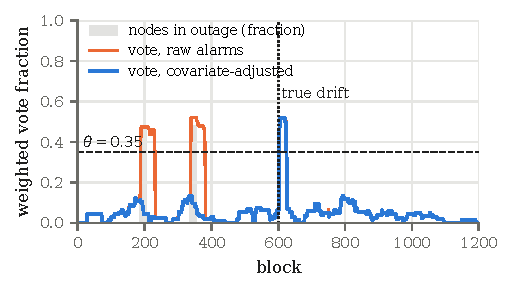
\includegraphics[width=\columnwidth]{fig1_motivation.pdf}
\caption{Vote counting cannot separate a shared outage from drift. One simulated run ($K=50$): two common-cause outages (grey) push the raw weighted vote (orange) above $\theta=0.35$ and would trigger two false federation-wide retrains; votes computed from covariate-adjusted alarms (blue) stay low during the outages and cross $\theta$ only at the true drift (block 600).}
\label{fig:motivation}
\end{figure}

\noindent\textbf{Shared external causes are common in edge fleets, and they are often recorded.} Power and backhaul outages affect every sensor behind a substation or gateway. Firmware rollouts and maintenance windows change many devices at once. Weather fronts affect outdoor sensors region by region. Industrial assets switch between operating modes. Supply voltage, link status, maintenance flags and operating settings are routinely logged as telemetry, but rules that count alarms ignore them.

\noindent\textbf{The difficulty is structural, not a tuning problem.} Raising $\theta$ above the share of weight a common cause can reach removes those false retrains, but it also misses every genuine drift that affects less weight. Our earlier version of this work proposed reliability-weighted Federated Drift Consensus (FDC) with an equal-weight Chernoff bound. That bound is invalid for heterogeneous weights, and an exponential-in-$K$ false-alarm guarantee cannot hold at all under common causes (Proposition~\ref{prop:limit}). Single-stream drift detectors such as ADWIN~\cite{bifet2007adwin}, DDM~\cite{gama2004ddm} and Page--Hinkley/CUSUM tests~\cite{page1954cusum} do not address this federation-level question. Drift-aware federated learning such as FedDrift~\cite{jothimurugesan2023feddrift} adapts models to drift but does not ask whether an apparent drift has an external common cause.

\noindent\textbf{Approach.} When the common cause is observed, for example supply voltage, uplink status or an operating mode recorded with the data, each node can test whether its alarm survives adjustment for that covariate before it votes. This is a backdoor adjustment~\cite{pearl2009causality} applied to a two-window change statistic. It costs one small regression per node and window and requires no causal-structure learning. We call the resulting decision layer, which combines reliability-weighted consensus, this common-cause-aware alarm filter and an anytime-valid detector, NeuroStream. The paper makes three contributions:
\begin{itemize}
\item[\textbf{C1}] \textbf{Theory of weighted vote counting.} A per-window false-alarm bound in the effective federation size $\Keff=(\sum_i\alpha_i)^2/\sum_i\alpha_i^2$ (Theorem~\ref{thm:keff}); a lower bound showing that no vote threshold controls false alarms under a common cause (Proposition~\ref{prop:limit}); and an anytime-valid average-run-length guarantee for an e-detector on the votes (Theorem~\ref{thm:arl}), which holds for covariate-adjusted votes and provably fails for raw ones. Evidence: Fig.~\ref{fig:theory}, \S\ref{sec:res-theory}.
\item[\textbf{C2}] \textbf{A common-cause-aware alarm filter}, evaluated against threshold tuning, local detectors and a FedDrift re-implementation: in a controlled simulation with known ground truth, on three public streams with labelled injected outages, and on a real recorded common cause (C-MAPSS operating conditions). Its failure modes are mapped: hidden, noisy or spoofed covariates and vote flooding. Evidence: Tables~\ref{tab:sim}--\ref{tab:cmapss}, Figs.~\ref{fig:tradeoff}--\ref{fig:real}.
\item[\textbf{C3}] \textbf{Accounting of privacy and robustness for the decision layer.} The accounting charges every data-dependent release, including the votes. A corrected Sparse-Vector vote is evaluated, and robust aggregators face adaptive attacks. Evidence: Fig.~\ref{fig:privacy}, \S\ref{sec:res-privacy}--\ref{sec:res-byz}.
\end{itemize}
\noindent\textbf{Scope.} The individual components (weighted voting, Hoeffding-type bounds, covariate adjustment, Rényi accounting, robust aggregation) are standard. What is new is how they are combined in the federated alarm-handling setting, the impossibility result that motivates the combination, and evidence of when it works and when it does not. Outages and drifts in the stream experiments are injected and labelled as such. We report no hardware, latency or energy measurements.

\section{Related Work}\label{sec:related}
\noindent\textbf{Drift detection.} Concept-drift detectors compare recent and reference statistics. ADWIN~\cite{bifet2007adwin} uses a Hoeffding cut over adaptive windows; DDM and EDDM~\cite{gama2004ddm,baena2006eddm} monitor error rates; CUSUM and Page--Hinkley tests~\cite{page1954cusum} accumulate evidence sequentially~\cite{gama2014survey}. All are single-stream methods. We use a fixed two-window Hoeffding test because it admits the analysis below, and we run ADWIN, DDM and Page--Hinkley from River~\cite{montiel2021river} as local baselines.

\noindent\textbf{Federated learning under drift.} FedAvg~\cite{mcmahan2017fedavg} and its successors assume a stationary objective; temporal shift is an open problem~\cite{kairouz2021advances}. FedDrift~\cite{jothimurugesan2023feddrift} detects drift at clients from accuracy drops, isolates drifted clients on new models and merges models by hierarchical clustering; later work clusters classifiers under distributed drift~\cite{chen2024fedccfa}. These methods decide \emph{how} to adapt. Our question is \emph{whether} an apparent federation-wide change warrants a federation-wide response. We re-implement FedDrift as a baseline and measure how it reacts to outages.

\noindent\textbf{Distributed change detection.} Quickest change detection in distributed sensor systems~\cite{tartakovsky2008distributed} and scalable monitoring of many streams~\cite{mei2010scalable} combine local statistics into a global decision, usually assuming that streams are independent given the change. Proposition~\ref{prop:limit} shows what goes wrong when a shared cause breaks that assumption, and Theorem~\ref{thm:arl} states the condition under which a federation-level guarantee is restored.

\noindent\textbf{Sequential and anytime-valid inference.} Ville's inequality~\cite{ville1939} underlies time-uniform confidence sequences~\cite{howard2021timeuniform} and e-value-based testing~\cite{ramdas2023gametheoretic}. E-detectors~\cite{shin2024edetectors} give change detectors with average-run-length guarantees. Theorem~\ref{thm:arl} instantiates a Shiryaev--Roberts e-detector with Hoeffding e-values on weighted votes. The new part is the identification of the condition (alarms independent given observed common causes) under which it is valid in a federation.

\noindent\textbf{Causal reasoning in federated settings.} Backdoor adjustment~\cite{pearl2009causality} and invariance-based methods~\cite{peters2016icp} separate mechanism changes from confounded associations. Federated causal discovery learns causal graphs from distributed data~\cite{ng2022federatedbn,gao2023feddag,li2024fcd}. We do not learn structure: we adjust for pre-specified observed covariates. Federated causal discovery is not new, and we claim nothing for it.

\noindent\textbf{Robust aggregation and differential privacy.} Coordinate-wise median and trimmed mean~\cite{yin2018byzantine}, Krum~\cite{blanchard2017krum}, FLTrust~\cite{cao2021fltrust} and centered clipping~\cite{karimireddy2021cclip} are evaluated against adaptive attacks~\cite{baruch2019alie,xie2020ipm,shejwalkar2021minmax}. For DP~\cite{dwork2006calibrating,dwork2014algorithmic} we use Rényi/zero-concentrated accounting~\cite{mironov2017renyi,bun2016zcdp} via \texttt{dp\_accounting}~\cite{dpaccounting} and the Sparse-Vector technique as analysed by Lyu et al.~\cite{lyu2017svt}. Data-dependent participation is an output that must be accounted for; the drafts preceding this paper omitted that cost.

\section{Problem Setting}\label{sec:setting}
\noindent\textbf{Federation and alarms.} Node $i\in\{1,\dots,K\}$ observes a stream in blocks $b=1,2,\dots$. Its detector compares the means of the last two sub-windows of $M_B$ blocks on $C$ monitored channels (records scaled to $[0,1]$, $m$ records per sub-window) and raises a raw alarm when $\max_c|\bar y^{\text{new}}_c-\bar y^{\text{old}}_c|>\epsilon_{\text{cut}}=\sqrt{\ln(4/\delta')/(2m)}$. The node's vote $d_i\in\{0,1\}$ for a decision window of $W$ blocks indicates an alarm within the window. The coordinator declares a global drift when $v=\sum_i\alpha_i d_i/\sum_i\alpha_i\ge\theta$. Node weights $\alpha_i$ are proportional to data volume. Table~\ref{tab:notation} lists the notation.

\noindent\textbf{Common causes.} An external variable $Z_t$, for example a regional supply sag, can shift the monitored statistics of many nodes at once without any change in the process the model serves. Each node records a covariate $z_i(t)$ (e.g., its supply voltage) that reflects $Z$ at that node.

\noindent\textbf{Threat and privacy model.} Up to a weight fraction $\beta_w$ of nodes may be Byzantine: they send arbitrary votes, covariates or model updates. Privacy is record-level $(\varepsilon,\delta)$-DP~\cite{dwork2006calibrating} of each node's records with respect to everything the node releases (votes, statistics, model updates). Covariates such as supply voltage are treated as non-sensitive device telemetry.

\begin{assumption}[null alarms]\label{as:null}
Absent a global drift, given the past and the observed covariates, the votes in a decision window are independent across nodes and $\sum_i\alpha_iP(d_i=1\mid\cdot)\le p\sum_i\alpha_i$.
\end{assumption}
\begin{assumption}[predictable weights]\label{as:weights} The $\alpha_i$ and $p$ are fixed before the window (measurable with respect to the past).\end{assumption}
\begin{assumption}[observed, adjustable common causes]\label{as:adjust} Every external cause that shifts the monitored statistics of more than one node is reflected in the observed $z_i$. Within a window its effect is linear in $z_i$, and genuine drift does not act through $z_i$ ($z_i$ is not a descendant of the drift).\end{assumption}
\begin{assumption}[bounded records]\label{as:bounded} Monitored records lie in $[0,1]$ (after clipping), which fixes Hoeffding cuts and DP sensitivities.\end{assumption}
\noindent Assumption~\ref{as:null} fails under common causes. Assumption~\ref{as:adjust} is what the filter needs, and \S\ref{sec:res-sim} measures what happens when it fails.

\begin{table}[t]\centering\small
\caption{Notation.}\label{tab:notation}
\begin{tabular}{@{}ll@{}}\toprule
$K$, $\Keff$ & nodes; effective size $(\sum\alpha_i)^2/\sum\alpha_i^2$\\
$\alpha_i$, $d_i$, $v$ & vote weight; vote; weighted vote fraction\\
$\theta$, $p$ & threshold; null mean alarm probability (A\ref{as:null})\\
$M_B$, $W$, $m$ & blocks per sub-window; decision window; records\\
$z_i$, $\beta_i$ & observed covariate; within-window slope\\
$\pi,\gamma,q$ & cause probability; affected weight; alarm prob.\\
$e_t$, $R_t$, $c$ & e-value; Shiryaev--Roberts statistic; threshold\\
$\varepsilon_{\text{svt}}$, $c_{\text{svt}}$ & Sparse-Vector budget and cutoff\\
$\sigma$, $R$ & noise multiplier; updates per retraining\\
\bottomrule\end{tabular}\end{table}

\section{Method}\label{sec:method}
\subsection{Weighted consensus and its limits}
\begin{theorem}[per-window bound]\label{thm:keff}
Under A\ref{as:null}--A\ref{as:weights}, for $\theta>p$: $P(v\ge\theta)\le\exp(-2\Keff(\theta-p)^2)$.
\end{theorem}
\noindent\emph{Proof sketch.} The terms $\alpha_id_i$ are independent and bounded in $[0,\alpha_i]$; Hoeffding's inequality~\cite{hoeffding1963} bounds $P(\sum\alpha_id_i-E\ge t)$ by $\exp(-2t^2/\sum\alpha_i^2)$ with $t=(\theta-p)\sum\alpha_i$. Full proof in Appendix~\ref{app:proofs}. With equal weights $\Keff=K$; with heterogeneous weights $\Keff<K$, and the equal-weight form used in our earlier draft is not a valid bound (Fig.~\ref{fig:theory}a).
\begin{proposition}[limit of vote counting]\label{prop:limit}
If a common cause with probability $\pi$ makes each node of a group holding weight fraction $\gamma$ alarm independently with probability at least $q$, and $\gamma q>\theta$, then $P(\text{false global})\ge\pi\,(1-\exp(-2\Keff(\gamma q-\theta)^2))\to\pi$ as $\Keff\to\infty$.
\end{proposition}
\noindent The false-alarm rate does not decay with federation size for any threshold $\theta<\gamma q$, and $\theta\ge\gamma q$ misses genuine drifts that affect less weight than $\gamma q$.

\begin{corollary}[Byzantine voters]\label{cor:byz}
If adversarial nodes hold weight fraction $\beta_w$ and the honest nodes satisfy A\ref{as:null} with effective size $\Keff^{H}$, then for $\theta-\beta_w>p(1-\beta_w)$: $P(v\ge\theta)\le\exp\!\big(-2\Keff^{H}(\theta-\beta_w-p(1-\beta_w))^2/(1-\beta_w)^2\big)$.
\end{corollary}

\subsection{Common-cause-aware alarm filter}
Each node regresses each monitored channel on its covariate $z_i$ over the current window of $2M_B$ blocks and re-applies the cut to the adjusted difference
$\Delta^{\text{adj}}_c=(\bar y^{\text{new}}_c-\bar y^{\text{old}}_c)-\hat\beta_c(\bar z^{\text{new}}-\bar z^{\text{old}})$, where $\hat\beta_c$ is the within-window least-squares slope. It votes $\tilde d_i=1$ only if both the raw and the adjusted tests fired within the decision window. All quantities are running sums, so the cost is $O(C)$ per node and block. Under A\ref{as:adjust}, $\Delta^{\text{adj}}$ removes the covariate-explained shift, and the filtered votes satisfy A\ref{as:null} with the filtered alarm probability $\tilde p$ (Proposition~\ref{prop:filtered}, Appendix~\ref{app:proofs}). Theorems~\ref{thm:keff} and~\ref{thm:arl} then apply to $\tilde v=\sum\alpha_i\tilde d_i/\sum\alpha_i$. When A\ref{as:adjust} fails, because the cause is hidden or the covariate is a poor proxy, Proposition~\ref{prop:limit} applies to the filtered votes as well.

\subsection{Anytime-valid declaration}
The threshold rule controls one window, but the coordinator tests every window, indefinitely. On disjoint epochs of $W$ blocks we form Hoeffding e-values $e_t=\frac{1}{|\Lambda|}\sum_{\lambda\in\Lambda}\exp(\lambda(v_t-p)-\lambda^2/(8\Keff))$ and the Shiryaev--Roberts statistic $R_t=(1+R_{t-1})e_t$, and declare when $R_t\ge c$, then reset.
\begin{theorem}[average run length]\label{thm:arl}
Under A\ref{as:null}--A\ref{as:weights} holding in every epoch, the first declaration time $\tau_c$ satisfies $E_\infty[\tau_c]\ge c$; after each reset the same holds, so false declarations occur at a long-run rate of at most $1/c$ per epoch.
\end{theorem}
\noindent\emph{Proof sketch.} Hoeffding's lemma gives $E[e_t\mid\mathcal F_{t-1}]\le1$, so $R_t-t$ is a supermartingale; optional stopping at $\tau_c\wedge n$ and Fatou's lemma give $c\le E[R_{\tau_c}]\le E[\tau_c]$ (Appendix~\ref{app:proofs}). Corollary~\ref{cor:arl-thr} in the appendix gives the analogous bound $\ARL\ge\exp(2\Keff(\theta-p)^2)$ for the threshold rule.

\subsection{Private votes and accounting}
Votes, filter statistics and model updates are all data-dependent releases. Each node privatises its vote with a Sparse-Vector gate~\cite{lyu2017svt} applied to its own covariate-adjusted statistic. The threshold noise is $\mathrm{Lap}(\Delta/\varepsilon_1)$, drawn once per instance; the query noise is $\mathrm{Lap}(2c_{\text{svt}}\Delta/\varepsilon_2)$; $\varepsilon_1=\varepsilon_2=\varepsilon_{\text{svt}}/2$ and $\Delta=1/m$. An instance halts after $c_{\text{svt}}$ positive answers. A positive answer puts the node in the voting state for $W$ blocks. Because the adjustment runs at the node, the filter adds no release. Each instance is $\varepsilon_{\text{svt}}$-DP, i.e.\ $\varepsilon_{\text{svt}}^2/2$-zCDP~\cite{bun2016zcdp}; a retraining consists of $R$ Gaussian releases with noise multiplier $\sigma$; all releases are composed in Rényi DP~\cite{mironov2017renyi} and converted to $(\varepsilon,\delta)$~\cite{canonne2020discrete}. The implementation in our earlier draft redrew the threshold noise after every positive answer while keeping the scales above. That combination costs $\frac{c_{\text{svt}}+1}{2}\varepsilon_{\text{svt}}$, not $\varepsilon_{\text{svt}}$, for $c_{\text{svt}}>1$; it is corrected here.

\begin{algorithm}[t]\small
\caption{Common-cause-aware FDC (one decision step)}\label{alg:fdc}
\begin{algorithmic}[1]
\Require weights $\alpha$; threshold $\theta$ or e-detector $(p,\Lambda,c)$; windows $M_B,W$
\State \textbf{at node $i$:} update running sums of $y$, $z$, $z^2$, $zy$
\State raw test $r_i\gets[\max_c|\Delta_c|>\epsilon_{\text{cut}}]$; adjusted test $a_i\gets[\max_c|\Delta^{\text{adj}}_c|>\epsilon_{\text{cut}}]$
\State vote $\tilde d_i\gets$ (any $r_i$ in last $W$) $\wedge$ (any $a_i$ in last $W$) \Comment{or SVT on $\Delta^{\text{adj}}$}
\State \textbf{at coordinator:} $\tilde v\gets\sum_i\alpha_i\tilde d_i/\sum_i\alpha_i$
\If{$\tilde v\ge\theta$ (or $R_t\ge c$ at an epoch end)} \textsc{global}: coordinated retraining ($R$ DP rounds); reset windows
\ElsIf{node $i$ alarmed in $r$ consecutive windows} \textsc{local}($i$): node-local retrain
\Else\ \textsc{none}: log suppressed episodes and the explaining covariate
\EndIf
\end{algorithmic}
\end{algorithm}

\noindent\textbf{Weights, calibration and cost.} Votes are weighted by data volume. A reliability factor (the share of a node's calibration-period alarms that survive adjustment, which needs no ground truth) is evaluated as an ablation. By A\ref{as:weights}, weights must be fixed before a window and must not depend on its votes. The bound $p$ for the e-detector is the weighted null alarm rate of the filtered votes, estimated on calibration runs, plus a margin of 0.02. The grid $\Lambda$ spans small to large shifts in vote fraction: the best single $\lambda$ for a shift $\Delta v$ is $4\Keff\Delta v$, and averaging e-values over $\Lambda$ keeps them valid. A node sends one bit (or one Sparse-Vector output) per decision window and keeps $O(C)$ running sums. The coordinator computes one weighted sum, plus $|\Lambda|$ exponentials per epoch for the e-detector. The \textsc{local} branch of Algorithm~\ref{alg:fdc} uses the same filtered alarms, so a node whose unexplained alarms persist for $r$ windows retrains on its own.

\noindent\textbf{Failure modes.} The filter can fail in four ways: a cause not reflected in any covariate (A\ref{as:adjust} fails; Proposition~\ref{prop:limit} returns); a covariate too noisy to estimate the slope; a covariate that is a descendant of the drift, so adjusting for it would hide real drift; and a shared covariate feed that an adversary controls. \S\ref{sec:res-sim} quantifies the first, second and fourth.

\section{Experimental Setup}\label{sec:setup}
\noindent\textbf{Three tracks.} \emph{Track S} is a controlled simulation with known ground truth ($K=50$, 1,200 blocks, three channels, $m=50{,}000$ records per sub-window, $\delta'=0.002$, $W=10$). It contains local sensor faults, common-cause outages on a fixed half of the nodes observed through a supply covariate, and a drift at block 600 on half of the nodes. \emph{Track A} uses three public streams (Table~\ref{tab:data}) partitioned across nodes, with labelled injected outages (a sensor offset on half of the features of affected nodes, observed through a synthetic supply covariate) and a labelled injected concept drift (label swap on half the input space of half the nodes). Natural drift is left untouched. \emph{Track B} uses NASA C-MAPSS~\cite{saxena2008cmapss}, whose three recorded operational settings are a real observed common cause of sensor shifts.

\noindent\textbf{Datasets.} All four datasets are public (Table~\ref{tab:data}). Elec2 records half-hourly prices and demand in the New South Wales electricity market~\cite{harries1999elec}; we use the normalised version distributed through MOA and OpenML (dataset 151)~\cite{moadatasets,openml151,vanschoren2013openml}. Covertype assigns each 30\,m cell of four Colorado wilderness areas one of seven forest cover types from cartographic variables~\cite{blackard2000covtype,ucicovtype}. Airlines asks whether a scheduled flight will be delayed; it is the classification version, distributed through MOA and OpenML (dataset 1169), of the flight data used by Ikonomovska et al.~\cite{ikonomovska2011fimt,gomes2017arf,openml1169}. C-MAPSS contains simulated run-to-failure trajectories of turbofan engines; FD002 and FD004 cover six operating conditions~\cite{saxena2008cmapss,nasacmapss}. Because the official hosts were unreachable from our build environment, we used copies from two GitHub mirrors at fixed commits~\cite{streamingdatasets,cmapssmirror}. Their SHA-256 hashes are released, and a script downloads and verifies exactly these files (Code and Data Availability). No dataset was resampled, extended or synthesised.

\begin{table*}[t]\centering\footnotesize\setlength{\tabcolsep}{3pt}
\caption{Datasets. All are public and none is redistributed: \texttt{data/fetch\_data.py} downloads the files used (GitHub mirrors at pinned commits~\cite{streamingdatasets,cmapssmirror}) and checks their SHA-256. Records and features are those of the files used; MB is their size (C-MAPSS: all 12 files). Licences as stated on the official pages, checked on 20 November 2026.}\label{tab:data}
\begin{tabular}{@{}L{1.85cm}rrrL{2.6cm}L{1.4cm}L{2.45cm}L{2.35cm}L{2.75cm}@{}}\toprule
dataset & records & feat. & MB & official source & licence & nodes, partition & events & preprocessing\\\midrule
Elec2~\cite{harries1999elec} & \RowsElec & \FeatElec & \BytesElec & OpenML 151~\cite{openml151}; MOA~\cite{moadatasets} & not stated [VERIFY] & $K\in\{5,10\}$; Dirichlet(0.5) label skew & natural; injected outages and drift & normalised file (no \emph{date}, \emph{day}); warm-up standardisation\\
Covertype~\cite{blackard2000covtype} & \RowsCov & \FeatCov & \BytesCov & UCI repository~\cite{ucicovtype}, doi:10.24432/\allowbreak C50K5N & CC BY 4.0 & $K\in\{10,50,100\}$; wilderness area & natural; injected outages and drift & warm-up standardisation\\
Airlines~\cite{ikonomovska2011fimt,gomes2017arf} & \RowsAir & \FeatAir & \BytesAir & OpenML 1169~\cite{openml1169}; MOA~\cite{moadatasets} & not stated [VERIFY] & $K\in\{10,50,100\}$; top-$K$ departure airports & natural; injected outages and drift & one-hot airline and weekday; time, length; warm-up standardisation\\
C-MAPSS FD002 / FD004~\cite{saxena2008cmapss} & \begin{tabular}[t]{@{}r@{}}\CmRowsTwo{} /\\ \CmRowsFour\end{tabular} & 14 & \BytesCm & NASA Open Data Portal~\cite{nasacmapss} & not specified on the portal & \EngTwo{} / \EngFour{} training engines$^{\ast}$, one per node & natural degradation; recorded operating condition & 14 sensors; standardised per operating condition (adjusted) or fleet-wide (raw)\\\bottomrule
\end{tabular}\\[2pt]
\parbox{\textwidth}{\footnotesize $^{\ast}$The dataset readme lists 248 training trajectories for FD004; \texttt{train\_FD004.txt} contains 249 unit IDs, which is the number we use.}
\end{table*}

\noindent\textbf{Paired counterfactual evaluation.} Every event type draws from its own random stream. For each seed we run the identical stream with and without the injected drift (and, in Track A, without the injected outages). A detection is \emph{attributable} only if the declaration is absent from the paired run, which prevents outage alarms from counting as drift detections. An outage-induced false retrain is a declaration episode present with the outages but absent without them.

\noindent\textbf{Injected events and what remains natural.} In Track A, outages start at rate 0.01 per block after a warm-up of 10\% of the stream, last 10 blocks, and hit each node of a fixed half of the federation with probability 0.9. The injected drift starts at two thirds of the stream. The model is softmax regression trained by FedAvg on the warm-up blocks; features are standardised with warm-up statistics only. The open loop freezes this model and scores three paired variants of the same stream: natural only, plus outages, and plus outages and drift. Their differences isolate the injected effects, while natural drift, which is present in all three variants, is reported separately. The closed loop lets each policy retrain the model. Appendix~\ref{app:repro} lists every parameter.

\noindent\textbf{Methods.} We run local retraining on every alarm (two-window, ADWIN, DDM, Page--Hinkley); FDC at fixed $\theta$ and at a threshold \emph{tuned on separate validation seeds} (lowest false-retrain rate subject to attributable detection $\ge0.9$); FDC with the filter, tuned the same way; the e-detector on raw and filtered votes; periodic and oracle retraining; and FedDrift, re-implemented from the official code (hierarchical variant, $\delta=\delta'=0.06$, every client starting on its own model, merging by complete linkage). The re-implementation runs on softmax regression and uses a 20-block history for cluster accuracies where the original uses all past data.

Local detectors use River's defaults except ADWIN ($\delta=0.002$). The same tuning rule and the same grid ($\theta\in\{0.15,\dots,0.55\}$ in Track A; $\{0.25,\dots,0.65\}$ in Track S) are applied to plain FDC and to the filter. The comparison is therefore between two tuned systems, not between a tuned system and a default.

\noindent\textbf{Metrics and statistics.} We report false global retrain episodes per 1,000 blocks (refractory $W$), attributable detection within a horizon, delay, wasted node-retrains, prequential accuracy, updates released per node, and $\varepsilon$ at $\delta=10^{-5}$. Track S uses 200 test seeds and 100 for sweeps; Track A uses 20 test and 10 validation seeds; the closed-loop and robustness runs use 10 seeds. Intervals are 95\%: bootstrap for means, Wilson for proportions, and exact Poisson upper bounds when no event occurred. No significance tests are reported.

\noindent\textbf{Compute.} All runs used a 2-vCPU sandbox without a GPU, Python 3.13, NumPy 2.5, River 0.27 and \texttt{dp\_accounting} 0.7. Every number in this paper is generated from seeded scripts by \texttt{exps/f\_numbers.py}.

\section{Results}\label{sec:results}
\subsection{The theory holds where its assumptions hold, and only there}\label{sec:res-theory}
\noindent\textbf{The corrected bound is valid; the equal-weight bound is not.} The equal-weight bound is violated in \LegViol{} of \LegN{} configurations, all with heterogeneous weights; the $\Keff$ bound in \LegCorrViol (Fig.~\ref{fig:theory}a). Under a common cause covering half the weight, the false-positive probability stays between \LegCCmin{} and \LegCCmax{} ($\pi=0.05$) for every $K$ from 10 to 400 (Fig.~\ref{fig:theory}b), as Proposition~\ref{prop:limit} predicts.

\noindent\textbf{The anytime guarantee holds for independent alarms and collapses under a common cause.} With independent alarms and heterogeneous weights, the empirical $\ARL$ of the e-detector exceeded $c$ in all \TindN{} configurations (Fig.~\ref{fig:theory}c). With a common cause occurring in 1\% of epochs, $\ARL$ stayed between \TccArlLo{} and \TccArlHi{} epochs for every $c$ up to 1,000, i.e.\ near $1/\pi$. In 20,000-block simulator runs with outages, raw votes produced a false declaration every \TlongRawArlLo--\TlongRawArlHi{} epochs. Filtered votes produced \TlongFilFAhundred{} false declarations in \TlongEpochs{} epochs at $c=100$, and \TlongFilFAc{} at $c=20$. Corollary~\ref{cor:byz} held in all \TbyzN{} Byzantine-weight configurations. When half the weight drifts, the e-detector's median delay is \TdelayHalf{} epoch(s) at $c=1000$.

\begin{figure*}[t]\centering
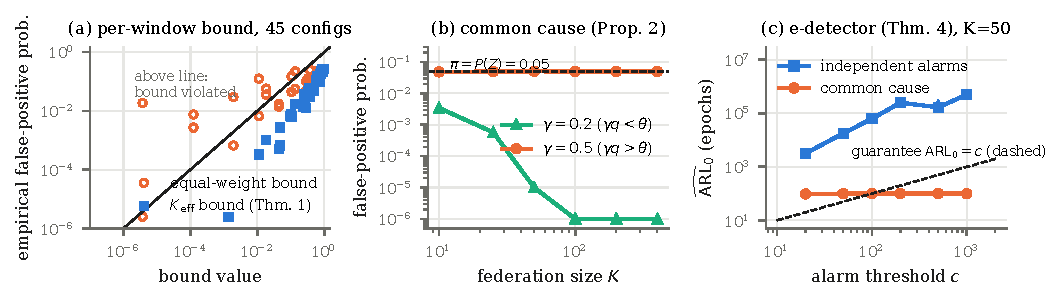
\includegraphics[width=\textwidth]{fig2_theory.pdf}
\caption{Theory vs.\ Monte Carlo. (a) The equal-weight bound is violated (points above the diagonal); the $\Keff$ bound is not. (b) A common cause covering weight $\gamma q>\theta$ keeps the false-positive probability at $\pi$ for all $K$; points at $10^{-6}$ are zero observed events. (c) The e-detector's $\widehat{\ARL}$ exceeds $c$ for independent alarms and is pinned near $1/\pi=100$ under a common cause; arrows mark lower bounds where no alarm occurred.}\label{fig:theory}
\end{figure*}

\subsection{Controlled simulation: the filter removes common-cause retrains that tuning cannot}\label{sec:res-sim}
\noindent\textbf{Main comparison.} Plain FDC at $\theta=0.35$ declares \SfdcFE{} \SfdcFEci{} false federation-wide retrains per 1,000 blocks, and its attributable detection is \SfdcDet{}. Counting outage flags as detections inflates the raw detection rate to \SfdcRawDet, the bias our paired evaluation removes (Table~\ref{tab:sim}). The threshold tuned on validation seeds ($\theta^\ast=\SthetaFdc$) lowers false retrains only to \SfdctFE. Raising $\theta$ to 0.55 cuts them to \SfdcHighFE{} but detects only \SfdcHighDet{} of drifts. With the filter, no false retrain occurred in 200 seeds (95\% upper bound \SfilUCB{} per 1,000 blocks), and attributable detection was \SfilDet{} \SfilDetci. Retraining every node on its own alarm wastes \SlocalW{} node-retrains per 1,000 blocks; filtering those local alarms leaves \SlocfilW{}, which are the genuine local faults. The e-detector on filtered votes had no false declaration and detected every drift; on raw votes it raised \SedRawFA{} false declarations per 1,000 epochs.

\begin{table}[t]\centering\scriptsize\setlength{\tabcolsep}{2.5pt}
\caption{Track S, outages + drift on 50\% of nodes, 200 test seeds. False retrains per 1,000 pre-drift blocks (95\% CI; Poisson upper bound when zero), attributable detection within 60 blocks (Wilson CI), wasted node-retrains per 1,000 blocks. $^\dagger$node-level detection; $^\ddagger$per 1,000 epochs.}\label{tab:sim}
\begin{tabular}{@{}lccc@{}}\toprule
method & false retrains & attrib.\ detection & wasted \\\midrule
\inputtable{tables/tab_sim_main.tex}
\bottomrule\end{tabular}\end{table}

\noindent\textbf{Weights and the local branch do not change the picture.} Equal weights give similar results (\WeqFdcFE{} false retrains for plain FDC). Volume $\times$ calibrated reliability lowers plain FDC to \WcalFdcFE{} at $\theta=0.35$ and \WcalFdcFEh{} at $\theta=0.45$ (detection \WcalFdcDeth), because that reliability estimate itself uses the covariate; the filter stays at zero (Appendix Table~\ref{tab:weights}). The \textsc{local} branch ($r=3$) triggered \SlocScopeF{} node-local retrains per 1,000 blocks with filtered alarms and \SlocScope{} with raw alarms. Most of them are the injected persistent local faults, which this branch is designed to handle. The filter's median detection delay was \SfilDelay{} blocks.

\noindent\textbf{No threshold reaches the filter's operating point.} Over $\theta\in[0.25,0.65]$, plain FDC trades false retrains against detection along one curve, while the filter's false-retrain rate never exceeds \CurveFilFEmax{} and its detection ranges from \CurveFilDetMin{} to \CurveFilDetMax{} with $\theta$ (Fig.~\ref{fig:tradeoff}a). These conclusions are unchanged for $K$ from 10 to 400, affected fractions from 0.4 to 1.0, drift magnitudes down to half the default, and all four weighting schemes (Appendix Tables~\ref{tab:sweeps}--\ref{tab:weights}). Plain FDC still produces \KfourFdcFE{} false retrains per 1,000 blocks at $K=400$: they do not decay with federation size, as Proposition~\ref{prop:limit} predicts. Two exceptions remain. With $K=10$ the filter left \KtenFilFE{} false retrains per 1,000 blocks. Drifts at one third of the default magnitude lower the filter's detection at $\theta=0.35$ to \MagLowFilDet{} (plain FDC: \MagLowFdcDet); at the tuned $\theta^\ast=\SthetaFil$ it recovers to \MagLowFiltTDet. Drifts affecting less weight than $\theta$ are, by definition, not detected as global.

\begin{figure*}[t]\centering
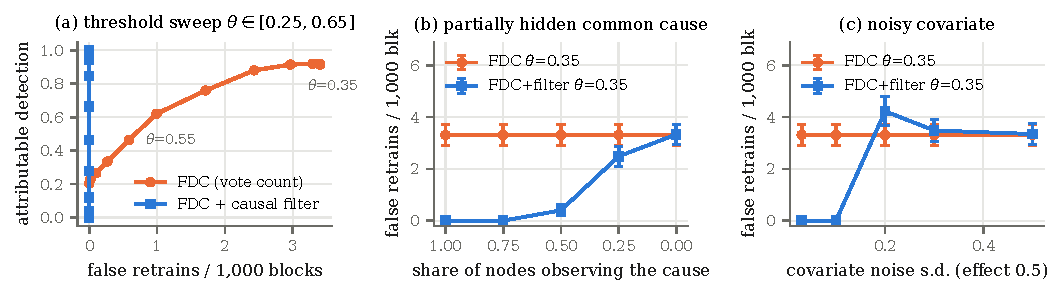
\includegraphics[width=\textwidth]{fig3_tradeoff_failure.pdf}
\caption{(a) Threshold sweep, 200 seeds: plain FDC cannot reach low false retrains without losing detection; the filter stays at zero false retrains. (b) When the covariate observes the outage at only part of the affected nodes, the advantage shrinks and vanishes for a hidden cause. (c) A covariate noise s.d.\ of 0.2 or more (outage effect 0.5) breaks the slope estimate; filtered declarations then flicker and can exceed plain FDC. Error bars: 95\% bootstrap CIs, 100 seeds.}\label{fig:tradeoff}
\end{figure*}

\noindent\textbf{The filter fails exactly where A\ref{as:adjust} fails, and it introduces one new attack surface.} If the covariate reflects the outage at only half of the affected nodes, false retrains rise to \SfailHalfFE; with a hidden cause, to \SfailHidFE, which equals plain FDC (Table~\ref{tab:failure}). A covariate noise level of 40\% of the outage effect raised filtered false retrains to \SfailNoiseFE, above plain FDC, because unstable slopes make declarations flicker. A non-linear covariate effect, where only severe sags shift the sensors, was still handled: \NonlinFilFE{} false retrains, against \NonlinFdcFE{} for plain FDC. A compromised shared covariate feed that reports an outage during a real drift lowered detection to \SspoofDet. Byzantine voters who always alarm were tolerated up to 10\% of nodes (\FloodOneFE{} false retrains); at 20\% and 30\% they caused \SfloodTwoFE{} and \SfloodThreeFE{} false retrains, consistent with Corollary~\ref{cor:byz} ($\beta_w<\theta-p$). Suppression by 30\% of nodes lowered detection to \SsuppThreeDet.

\begin{table*}[t]\centering\scriptsize\setlength{\tabcolsep}{4pt}
\caption{Track S failure modes and attacks on the decision layer (100 seeds; $\theta=0.35$). False = false global retrains per 1,000 blocks (95\% CI; Poisson upper bound when zero); detect = attributable detection (Wilson CI).}\label{tab:failure}
\begin{tabular}{@{}lcccc@{}}\toprule
& \multicolumn{2}{c}{FDC} & \multicolumn{2}{c}{FDC + filter}\\\cmidrule(lr){2-3}\cmidrule(lr){4-5}
condition & false & detect & false & detect\\\midrule
\inputtable{tables/tab_sim_failure.tex}
\bottomrule\end{tabular}\end{table*}

\subsection{Real streams with injected outages}\label{sec:res-real}
\noindent\textbf{Open loop: fewer outage-induced retrains, sometimes at a detection cost.} With thresholds tuned on validation seeds, the filter had fewer outage-induced false retrains than tuned FDC in \AnLower{} of \AnSettings{} dataset--size settings (Table~\ref{tab:real}, Fig.~\ref{fig:real}). Tuned FDC ranged from \AfdcFEmin{} to \AfdcFEmax{} per 1,000 blocks; the filter from \AfilFEmin{} to \AfilFEmax. Detection was equal or higher with the filter in \AnDetGeq{} settings and lower in \AnDetLower; the largest drop was in \AworstName{}, from \AworstDetF{} to \AworstDetC. Elec2 is too small for reliable federated detection at either threshold (\ElecRecFive{} to \ElecRecTen{} records per node and block). In \AgridEdge{} of the 16 tuned thresholds the selection hit the lower grid edge (\AgridMin).

\begin{figure}[t]\centering
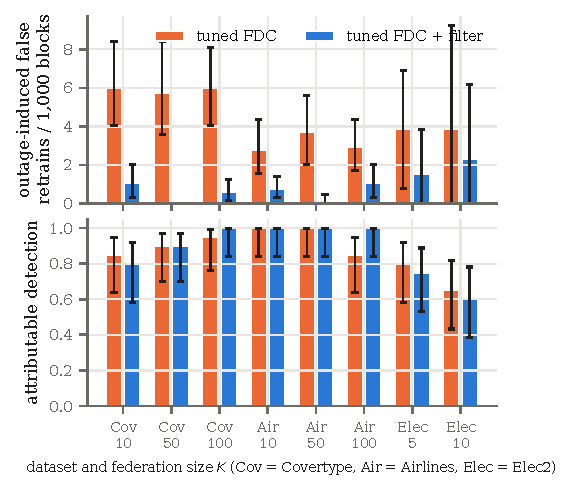
\includegraphics[width=\columnwidth]{fig4_real_streams.pdf}
\caption{Real streams with labelled injected outages and drift (20 test seeds; thresholds tuned on 10 validation seeds). Top: outage-induced false federation-wide retrains. Bottom: attributable detection of the injected drift. Error bars: 95\% CIs.}\label{fig:real}
\end{figure}

\begin{table*}[t]\centering\scriptsize\setlength{\tabcolsep}{3pt}
\caption{Track A, open loop (frozen warm-up model). False = outage-induced false global retrains per 1,000 blocks; detection = attributable detection within 30 blocks; local = outage-induced alarms of local two-window detectors per 1,000 blocks (summed over nodes). 20 test seeds; 95\% CIs.}\label{tab:real}
\begin{tabular}{@{}lccccccc@{}}\toprule
dataset & $K$ & $\theta^\ast$ FDC / filter & false, FDC & false, filter & detection, FDC & detection, filter & local \\\midrule
\inputtable{tables/tab_real_open.tex}
\bottomrule\end{tabular}\end{table*}

\noindent\textbf{Closed loop: the filter halves outage-coincident retrains without changing accuracy.} We inject a federation-wide drift and let each policy trigger retraining: ten FedAvg rounds on the last ten blocks (Table~\ref{tab:closed}). On both streams most retrains are triggered by natural drift, which is genuine: event-triggered retraining beats the static model on Covertype (\CovClFdcAcc{} vs.\ \CovClStaAcc). The filter reduced retrains that started during an outage from \CovClFdcOut{} to \CovClFilOut{} per run on Covertype and from \AirClFdcOut{} to \AirClFilOut{} on Airlines. Total retrains fell from \CovClFdcTot{} to \CovClFilTot{} and from \AirClFdcTot{} to \AirClFilTot. Overall accuracy changed by at most \ClAccDiffMax{} (\CovClFdcAcc{} vs.\ \CovClFilAcc; \AirClFdcAcc{} vs.\ \AirClFilAcc). In this setting the filter saves cost; it does not improve accuracy. FedDrift, which trains several models every block, was the most accurate (\CovClFdAcc{} and \AirClFdAcc), at \CovClFdRel{} update releases per node versus \CovClFilRel{} and \AirClFilRel{} for the filter. Before the drift, FedDrift's accuracy-drop rule fired on \CovClFdIsoPct\% and \AirClFdIsoPct\% of client-blocks. We kept the official $\delta=0.06$, and per-block accuracy on 10--20 records is noisy. Local ADWIN retraining (\CovClLocAcc, \AirClLocAcc) matched or slightly exceeded event-triggered global retraining without releasing updates, but it maintains one model per node. If continuous training is affordable, multi-model adaptation is the better choice. The filter is aimed at the regime in which every federated round is costly in compute or privacy budget.

\begin{table*}[t]\centering\scriptsize\setlength{\tabcolsep}{3pt}
\caption{Track A, closed loop ($K=50$, injected federation-wide drift, 10 seeds). Prequential accuracy before/after the drift and overall (95\% CI); retrains started before the drift ($^\S$client isolations before the drift for FedDrift); retrains started while an outage was active; model-update releases per node.}\label{tab:closed}
\begin{tabular}{@{}llcccccc@{}}\toprule
data & policy & acc.\ pre & acc.\ post & acc.\ all & retrains pre-drift & retrains in outage & releases/node \\\midrule
\inputtable{tables/tab_real_closed.tex}
\bottomrule\end{tabular}\end{table*}

\subsection{A real observed common cause: C-MAPSS operating conditions}\label{sec:res-cmapss}
\noindent\textbf{Conditioning on the recorded operating condition is what makes degradation detectable.} In FD002 and FD004, six operating conditions shift every sensor (Table~\ref{tab:cmapss}). Engines are not synchronised, so this is a node-level test. Without conditioning, the condition-driven variance masks degradation: only \CmRawDetTwo{} (FD002) and \CmRawDetFour{} (FD004) of engines alarm in their last 30 cycles. After per-condition normalisation estimated on the first 30 cycles, detection is \CmAdjDetTwo{} and \CmAdjDetFour, with healthy-region alarm rates of \CmAdjFATwo\% and \CmAdjFAFour\% of windows. Here the observed common cause costs detection power rather than causing false alarms, because conditions are drawn independently at each cycle and do not persist.

\begin{table}[t]\centering\scriptsize\setlength{\tabcolsep}{2pt}
\caption{C-MAPSS training trajectories. Healthy = RUL $>125$ cycles, degraded = RUL $\le30$; two-window test, $M_B=15$ cycles, Bonferroni over 14 sensors.}\label{tab:cmapss}
\begin{tabular}{@{}llcc@{}}\toprule
subset & detector & healthy alarms (\%) & degraded detection\\\midrule
\inputtable{tables/tab_cmapss.tex}
\bottomrule\end{tabular}\end{table}

\subsection{Privacy: false retrains are what exhausts the budget}\label{sec:res-privacy}
\noindent\textbf{The accountant matters, and so do the votes.} Under the earlier draft's setting ($\sigma=25$, release every round), basic, advanced, Rényi and PLD accounting give \AccBasic, \AccAdv, \AccRdp{} and \AccPld{} rounds before $\varepsilon>4$. Node-side Sparse-Vector votes with $\varepsilon_{\text{svt}}=0.2$, $c_{\text{svt}}=1$ preserve the filter's behaviour: zero false retrains, detection \SvtFilDet. The adjusted statistic triggers fewer positive answers than the raw one (\SvtPosFil{} vs.\ \SvtPosRaw{} per node per 1,000 blocks), so voting costs $\varepsilon=\SvtEpsRun$ per 1,200 blocks. Releasing DP-noised window sums to the coordinator instead needs noise multiplier 10 to remain accurate and costs $\varepsilon=\PfEpsTen$ over the same run. At multiplier 30 ($\varepsilon=\PfEpsThirty$) the slope estimate breaks and false retrains return to \PfFEThirty. Running the adjustment at the node and privatising only the vote is therefore the better design. Larger Sparse-Vector cutoffs are not a free saving: with $c_{\text{svt}}=5$ at $\varepsilon_{\text{svt}}=0.2$ the query noise makes the gate active in \SvtCfiveAct{} of blocks and raises plain FDC's false retrains to \SvtCfiveFE.

\noindent\textbf{With fewer false retrains, the budget lasts longer.} With $\sigma=10$, ten DP rounds per retraining and one genuine drift per 1,000 blocks, a node exhausts $\varepsilon=4$ after \HorCont{} blocks of continuous training, \HorPer{} with periodic retraining, \HorFdc{} with plain FDC and \HorFil{} with the filter, against \HorOra{} for an oracle (Fig.~\ref{fig:privacy}a). On our tasks the noise level is not what limits model quality; clipping is. On Covertype, clip-only training reaches \DpCovClip{} and training with $\sigma=10$ reaches \DpCovTen{} ($\varepsilon=\DpEpsTen$ after 60 rounds), against \DpCovZero{} without clipping (Appendix Table~\ref{tab:dputil}). With thousands of records per node, the noise on a summed gradient is small relative to the signal. The earlier claim that drift-gated participation ``costs zero budget'' is false. Once the gate is charged, a node-level gate extends the horizon by \GateGainRtwenty--\GateGainRone$\times$ at $\varepsilon_{\text{svt}}=0.2$ and $\sigma=25$, depending on how many releases one activation authorises ($R=20$ to $1$). It shortens the horizon at $\varepsilon_{\text{svt}}\ge0.5$ with $c_{\text{svt}}=1$ (Appendix Table~\ref{tab:gating}).

\begin{figure*}[t]\centering
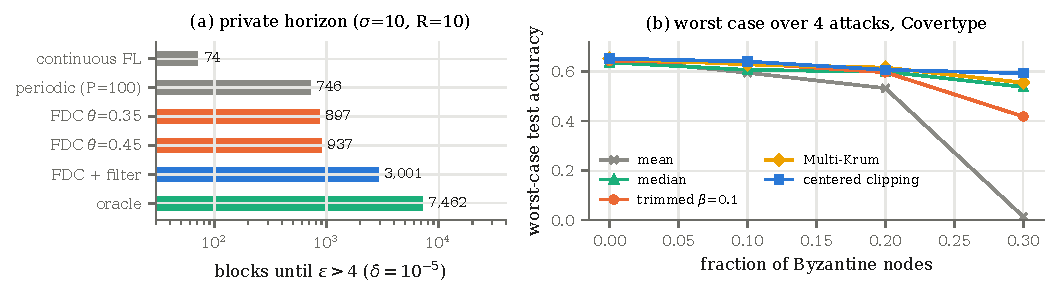
\includegraphics[width=\textwidth]{fig5_privacy_robustness.pdf}
\caption{(a) Blocks until a node's $\varepsilon$ exceeds 4 ($\delta=10^{-5}$) with $\sigma=10$, $R=10$ DP rounds per retraining and one genuine drift per 1,000 blocks, using measured Track S rates of false retrains and Sparse-Vector positives (log scale). (b) Covertype FedAvg test accuracy, worst case over four omniscient attacks (sign-flip, ALIE, IPM, min-max), $K=50$, IID partition, 10 seeds.}\label{fig:privacy}
\end{figure*}

\subsection{Robust aggregation under adaptive attacks}\label{sec:res-byz}
\noindent\textbf{Aggregation needs its own defence; the filter does not provide one.} On Covertype with $K=50$ and an IID partition, plain averaging reaches \ByzMeanNone{} without attack (Fig.~\ref{fig:privacy}b; full results in Appendix Table~\ref{tab:byz}). Over the four attacks at 30\% Byzantine nodes, the worst-case accuracy was \ByzTrimWorst{} for the trimmed mean, \ByzMedWorst{} for the median and \ByzBestWorst{} for the most robust aggregator, \ByzBestAgg. Under the wilderness-area partition, every aggregator stayed near the majority-class rate even without attack, so that run could not discriminate between aggregators; we report it in the result files only. The aggregator is orthogonal to the decision layer: the filter protects \emph{when} the federation retrains, not \emph{what} it learns.

\section{Limitations}\label{sec:limits}
\noindent (i)~Outages and drifts in the real streams are injected, and their covariate is synthetic. The only real recorded common cause we evaluate is C-MAPSS, and only at node level. We could not retrieve the Intel Berkeley Lab sensor data, so it is not evaluated. (ii)~The filter requires the common cause to be observed and its effect to be roughly linear within a window. It fails gracefully when the cause is partially hidden and badly when the covariate is noisy (Fig.~\ref{fig:tradeoff}). (iii)~Adjusting for a covariate that is itself affected by the drift would suppress genuine drift; this has to be ruled out per deployment. (iv)~A shared covariate feed is a single point of failure. (v)~Theorem~\ref{thm:arl} needs disjoint epochs and a valid null bound $p$; we calibrate $p$ on validation runs. (vi)~We do not measure hardware cost, latency or energy, and we used GitHub mirrors of the datasets; checksums are released, but the files have not yet been cross-checked against the official sources. (vii)~The FedDrift baseline is a re-implementation on softmax regression with a 20-block history, and its threshold $\delta$ was not re-tuned for our block sizes.

\section{Conclusion}\label{sec:conclusion}
Counting how many nodes alarm cannot separate drift from a shared external cause, and no threshold or federation size fixes this. When the cause is observed, covariate adjustment before voting restores the per-window and anytime-valid false-alarm guarantees. In our experiments it removed most outage-induced federation-wide retrains, and it extended the private training horizon because the budget is no longer spent on false retrains. The approach depends on the covariate: when the cause is hidden, noisy or spoofed, it is no better than counting. Accounting that charges every release, votes included, shows the practical gain: fewer false retrains leave more of each node's budget for genuine ones. The filter does not protect the model from Byzantine updates, and vote flooding or a spoofed covariate feed defeats it, so it has to be paired with a robust aggregator and an authenticated covariate source. The most important test still missing is a deployment log in which a real, recorded common cause triggers alarms across nodes.

\section*{Code and Data Availability}
\noindent\textbf{Code.} All code, configurations, seeds, per-seed result logs and the scripts that regenerate every number, table and figure in this paper are available at \RepoURL{} and archived on Zenodo (DOI: \ZenodoDOI). \texttt{make all} reproduces the full study; Appendix~\ref{app:repro} lists runtimes and library versions.

\noindent\textbf{Data.} The study uses only public datasets; no new data were collected and no dataset is redistributed. Official sources: Elec2, OpenML dataset 151 (\url{https://www.openml.org/d/151}) and the MOA dataset page (\url{https://moa.cms.waikato.ac.nz/datasets/})~\cite{harries1999elec,openml151,moadatasets}; Covertype, UCI Machine Learning Repository (\url{https://doi.org/10.24432/C50K5N}, CC BY 4.0)~\cite{blackard2000covtype,ucicovtype}; Airlines, OpenML dataset 1169 (\url{https://www.openml.org/d/1169}) and the MOA dataset page~\cite{ikonomovska2011fimt,openml1169,moadatasets}; NASA C-MAPSS, NASA Open Data Portal (\url{https://data.nasa.gov/dataset/cmapss-jet-engine-simulated-data})~\cite{saxena2008cmapss,nasacmapss}. The files used are copies from \url{https://github.com/scikit-multiflow/streaming-datasets} (commit \texttt{f1eb9f0}) and \url{https://github.com/edwardzjl/CMAPSSData} (commit \texttt{ed40e40}). Their SHA-256 hashes are listed in \texttt{data/SHA256SUMS.mirror}, and \texttt{python data/fetch\_data.py} downloads and verifies them. Injected outages and drifts are generated by the released, seeded code.

\section*{Acknowledgments}
The authors thank the maintainers of the public datasets used in this study: the UCI Machine Learning Repository (Covertype), the NASA Prognostics Center of Excellence (C-MAPSS), and the MOA and OpenML projects (Elec2 and Airlines), as well as the developers of the open-source libraries River and dp-accounting. This research received no specific grant from any funding agency in the public, commercial or not-for-profit sectors; the work was carried out entirely by the four authors.

\bibliographystyle{unsrt}
\ifdefined\ieeemode\bibliography{refs}\else{\small\bibliography{refs}}\fi % IEEEtran sets its own reference size

\appendix
\section{Proofs}\label{app:proofs}
\noindent Throughout, $A=\sum_i\alpha_i$, $Q=\sum_i\alpha_i^2$, $\Keff=A^2/Q$, $S=\sum_i\alpha_id_i$ and $v=S/A$.

\begin{proof}[Proof of Theorem~\ref{thm:keff}]
Under A\ref{as:null}--A\ref{as:weights} the terms $\alpha_id_i\in[0,\alpha_i]$ are conditionally independent and $E[S]\le pA$. Hoeffding's inequality~\cite{hoeffding1963} gives $P(S-E[S]\ge t)\le\exp(-2t^2/Q)$ for $t>0$. The event $\{S\ge\theta A\}$ implies $S-E[S]\ge(\theta-p)A$. With $t=(\theta-p)A$ we get $\exp(-2(\theta-p)^2A^2/Q)=\exp(-2\Keff(\theta-p)^2)$.
\end{proof}

\begin{proof}[Proof of Proposition~\ref{prop:limit}]
Condition on the cause $Z$. Let $G$ be the affected group and $S_G=\sum_{i\in G}\alpha_id_i\le S$. Given $Z$, $E[S_G]\ge q\gamma A$. The event $\{S<\theta A\}$ implies $S_G-E[S_G]<-(\gamma q-\theta)A$, whose probability is at most $\exp(-2(\gamma q-\theta)^2A^2/\sum_{G}\alpha_i^2)\le\exp(-2\Keff(\gamma q-\theta)^2)$ by Hoeffding, since $\sum_G\alpha_i^2\le Q$. Hence $P(S\ge\theta A\mid Z)\ge1-\exp(-2\Keff(\gamma q-\theta)^2)$; multiplying by $P(Z)=\pi$ gives the claim.
\end{proof}

\begin{proof}[Proof of Corollary~\ref{cor:byz}]
Write $S=S_H+S_B$ with $S_B\le\beta_wA$. Then $\{S\ge\theta A\}\subseteq\{S_H\ge(\theta-\beta_w)A\}$, while $E[S_H]\le pA_H$ with $A_H=(1-\beta_w)A$. Hoeffding over the honest nodes, with deviation $A(\theta-\beta_w-p(1-\beta_w))>0$, gives $\exp(-2A^2(\theta-\beta_w-p(1-\beta_w))^2/Q_H)$. Using $A^2=A_H^2/(1-\beta_w)^2$ and $\Keff^H=A_H^2/Q_H$ gives the stated form.
\end{proof}

\begin{proof}[Proof of Theorem~\ref{thm:arl}]
Fix $\lambda\ge0$. Under A\ref{as:null}--A\ref{as:weights} in epoch $t$, $v_t=\sum_i(\alpha_i/A)d_i$ is a sum of conditionally independent terms in $[0,\alpha_i/A]$ with $E[v_t\mid\mathcal F_{t-1}]\le p$. By Hoeffding's lemma, $E[\exp(\lambda(v_t-E[v_t\mid\mathcal F_{t-1}]))\mid\mathcal F_{t-1}]\le\exp(\lambda^2\sum_i\alpha_i^2/(8A^2))=\exp(\lambda^2/(8\Keff))$. Since $\lambda\ge0$ and $E[v_t\mid\mathcal F_{t-1}]\le p$, $E[\exp(\lambda(v_t-p)-\lambda^2/(8\Keff))\mid\mathcal F_{t-1}]\le1$, and the same holds for the average over $\lambda\in\Lambda$. So $E[e_t\mid\mathcal F_{t-1}]\le1$. With $R_0=0$, $E[R_t\mid\mathcal F_{t-1}]=(1+R_{t-1})E[e_t\mid\mathcal F_{t-1}]\le1+R_{t-1}$, so $M_t=R_t-t$ is a supermartingale with $M_0=0$. For the bounded stopping time $\tau_c\wedge n$, optional stopping gives $E[R_{\tau_c\wedge n}]\le E[\tau_c\wedge n]$. If $E[\tau_c]=\infty$ there is nothing to prove. Otherwise $\tau_c<\infty$ a.s. and $R_{\tau_c}\ge c$, and Fatou's lemma gives $c\le E[R_{\tau_c}]\le\liminf_nE[R_{\tau_c\wedge n}]\le\liminf_nE[\tau_c\wedge n]=E[\tau_c]$. After a reset the argument applies conditionally on the past, so each inter-declaration time has conditional expectation at least $c$.
\end{proof}

\begin{corollary}[threshold rule over time]\label{cor:arl-thr}
If A\ref{as:null}--A\ref{as:weights} hold in every disjoint epoch, the rule ``declare when $v_t\ge\theta$'' has conditional per-epoch false-alarm probability at most $q=\exp(-2\Keff(\theta-p)^2)$. The first false declaration $\tau$ therefore satisfies $P(\tau>t)\ge(1-q)^t$ and $E[\tau]\ge1/q$, and $P(\text{any false declaration in }T\text{ epochs})\le Tq$.
\end{corollary}
\begin{proof}
Theorem~\ref{thm:keff} holds conditionally on $\mathcal F_{t-1}$. Hence $P(\tau>t)=E[\prod_{s\le t}(1-P(v_s\ge\theta\mid\mathcal F_{s-1}))]\ge(1-q)^t$, and $E[\tau]=\sum_{t\ge0}P(\tau>t)\ge1/q$. The last claim is a union bound.
\end{proof}

\begin{proposition}[filtered votes]\label{prop:filtered}
Suppose A\ref{as:adjust} holds with the true within-window slope. Then, absent drift, each node's adjusted statistic is a function of its own observation noise only and its distribution does not depend on $Z$. The filtered votes are therefore conditionally independent given $Z$, with a mean alarm probability $\tilde p$ that does not depend on $Z$, and Theorems~\ref{thm:keff} and~\ref{thm:arl} hold for $\tilde v$ with $p$ replaced by $\tilde p$. With an estimated slope, $\tilde p$ also absorbs the estimation error; we calibrate it on validation runs (Track S: \SpFil{} for filtered vs.\ \SpRaw{} for raw alarms per window).
\end{proposition}
\begin{proof}[Proof sketch]
Under A\ref{as:adjust}, $y=\mu+\beta z+\eta$ within the window, with node-specific noise $\eta$ independent across nodes given $Z$. The adjusted difference with the true $\beta$ equals the difference of window means of $\eta$, which involves neither $z$ nor $Z$. Independence across nodes then follows from that of $\eta$.
\end{proof}

\section{Additional Results}\label{app:more}
This appendix gives the full results summarised in Section~\ref{sec:results}: robust aggregation under adaptive attacks (Table~\ref{tab:byz}), the Track S sweeps and weighting schemes (Tables~\ref{tab:sweeps} and~\ref{tab:weights}), the private training horizon and node-level gating (Tables~\ref{tab:horizon} and~\ref{tab:gating}), and the utility of differentially private training (Table~\ref{tab:dputil}).

\begin{table*}[!t]\centering\small
\caption{Robust aggregation on Covertype ($K=50$, IID partition, 40 rounds, omniscient attackers, 10 seeds): test accuracy without attack and under each attack with 20\% and 30\% Byzantine nodes.}\label{tab:byz}
\begin{tabular*}{\textwidth}{@{\extracolsep{\fill}}lccccccccc@{}}\toprule
aggregator & no attack & \multicolumn{2}{c}{sign-flip $\times3$} & \multicolumn{2}{c}{ALIE} & \multicolumn{2}{c}{IPM ($\epsilon=0.5$)} & \multicolumn{2}{c}{min-max}\\\cmidrule(lr){3-4}\cmidrule(lr){5-6}\cmidrule(lr){7-8}\cmidrule(lr){9-10}
& & 20\% & 30\% & 20\% & 30\% & 20\% & 30\% & 20\% & 30\%\\\midrule
\inputtable{tables/tab_byz.tex}
\bottomrule\end{tabular*}\end{table*}

\begin{table}[!tbp]\centering\scriptsize\setlength{\tabcolsep}{2pt}
\caption{Track S sweeps (100 seeds, $\theta=0.35$): false retrains / 1,000 blocks and attributable detection.}\label{tab:sweeps}
\resizebox{\columnwidth}{!}{%
\begin{tabular}{@{}lcccc@{}}\toprule
& \multicolumn{2}{c}{FDC} & \multicolumn{2}{c}{FDC + filter}\\\cmidrule(lr){2-3}\cmidrule(lr){4-5}
setting & false & detect & false & detect\\\midrule
\inputtable{tables/tab_sim_sweeps.tex}
\bottomrule\end{tabular}}\end{table}

\begin{table}[!tbp]\centering\scriptsize\setlength{\tabcolsep}{2pt}
\caption{Track S, weighting schemes (200 seeds, $\theta=0.35$). ``Calibrated $\rho$'' is the share of a node's calibration-period alarms that survive covariate adjustment; it uses no ground truth.}\label{tab:weights}
\resizebox{\columnwidth}{!}{%
\begin{tabular}{@{}lcccc@{}}\toprule
weights & FDC false & FDC detect & filter false & filter detect\\\midrule
\inputtable{tables/tab_sim_weights.tex}
\bottomrule\end{tabular}}\end{table}

\begin{table}[!tbp]\centering\footnotesize\setlength{\tabcolsep}{2.5pt}
\caption{Blocks until $\varepsilon>4$ ($\delta=10^{-5}$) per node: continuous training, periodic retraining every 100 blocks, plain FDC ($\theta=0.35$, $0.45$) and FDC + filter, each with $R=10$ DP rounds per retraining and Sparse-Vector votes ($\varepsilon_{\text{svt}}=0.2$). Retrain and vote rates measured in Track S.}\label{tab:horizon}
\begin{tabular*}{\columnwidth}{@{\extracolsep{\fill}}rrrrrrrr@{}}\toprule
$\sigma$ & $R$ & drifts/1k & cont. & periodic & FDC .35 & FDC .45 & filter\\\midrule
\inputtable{tables/tab_horizon.tex}
\bottomrule\end{tabular*}\end{table}

\begin{table}[!tbp]\centering\footnotesize\setlength{\tabcolsep}{2.5pt}
\caption{Node-level drift gating with the gate charged ($\sigma=25$; horizon without gating = \GateHorNoGate{} rounds). $R$ = releases authorised per positive Sparse-Vector answer. The earlier draft's analysis implicitly fixed $R=1$ and used the active-block fraction as the release fraction.}\label{tab:gating}
\begin{tabular*}{\columnwidth}{@{\extracolsep{\fill}}rrrrrrr@{}}\toprule
$\varepsilon_{\text{svt}}$ & $c_{\text{svt}}$ & $R$ & active frac. & positives/1k & horizon & gain\\\midrule
\inputtable{tables/tab_gating.tex}
\bottomrule\end{tabular*}\end{table}

\begin{table}[!tbp]\centering\footnotesize\setlength{\tabcolsep}{3pt}
\caption{Test accuracy of federated softmax regression: non-private (no clipping), clipping only ($C=1$), and DP with noise multiplier $\sigma$ (one full-batch step per round, 60 rounds, no subsampling; learning rate for clipped runs chosen on a validation seed: \DpLrCov{} for Covertype; 10 seeds). With one local step and weighted averaging, non-private FedAvg equals full-batch gradient descent and does not depend on the partition seed. Last row: record-level $\varepsilon$ per node at $\delta=10^{-5}$.}\label{tab:dputil}
\begin{tabular*}{\columnwidth}{@{\extracolsep{\fill}}lccccc@{}}\toprule
& non-private & clip only & $\sigma=1$ & 10 & 25\\\midrule
\inputtable{tables/tab_dputil.tex}
\bottomrule\end{tabular*}\end{table}

\section{Experimental Details and Reproducibility}\label{app:repro}
\noindent\textbf{Track S generator.} $K=50$; $C=3$ channels; block means of 5,000 records with per-record s.d.\ 0.25; node offsets $\mathcal N(0,0.05^2)$. Local faults: rate 0.001 per node-block, duration 20, shift 0.03 on one channel. Outages: start rate 0.004 per block on a fixed half of the nodes, each hit with probability 0.9, duration 20, shift 0.03 on channel 2. Covariate: $z=1-0.5\cdot\text{outage}+\mathcal N(0,0.03^2)$, clipped to $[0,1.5]$. Drift: shift 0.03 on channel 1 of half the nodes from block 600. Detector: $M_B=10$, $\delta'=0.002$, $\epsilon_{\text{cut}}=0.0087$, $W=10$. Weights: data volume $\sim\mathrm{LogNormal}(0,0.5)$. Separate random streams per event type (\texttt{numpy.random.SeedSequence.spawn}). Seeds: test 0--199, validation 1000--1099 (tuning), calibration of $p$ for the e-detector on seeds 1000--1029, long-horizon runs 5000--5009. E-detector: $\Lambda=\{5,10,20,40,80\}$; $p$ = calibrated weighted epoch-alarm rate + 0.02.

\noindent\textbf{Track A.} Rows in original order are split into 600 blocks (Elec2: 150). The first 10\% of blocks are warm-up: 30 FedAvg rounds of softmax regression (5 local gradient steps, learning rate 0.5); features are standardised using warm-up statistics only. Outages: start rate 0.01 per block after warm-up on a fixed half of the nodes, hit probability 0.9, duration 10 blocks, offset $+3$ on a fixed random half of the standardised features. The covariate is synthetic: $z=1-0.5\cdot\text{outage}+\mathcal N(0,0.03^2)$. Injected drift at block $0.67B$ on half the nodes: classes 0 and 1 are swapped for records whose drift feature (Elec2 \emph{period}, Covertype \emph{Elevation}, Airlines \emph{Time}) is above its warm-up median. Detector: one-sided two-window test on pooled error rates with the ADWIN harmonic-mean cut. Closed loop: federation-wide drift ($\gamma=1$); a retraining runs 10 FedAvg rounds on each node's last 10 blocks; refractory period 10 blocks; periodic $P=50$; local ADWIN ($\delta=0.002$) retrains a node's own model.

\noindent\textbf{Reproducibility checklist.} Code, configurations and seeds: \texttt{ns/}, \texttt{exps/}. Per-seed logs, configuration hashes and library versions: \texttt{results/**/*.json}. Repository: \RepoURL{} (archived release: \ZenodoDOI). Data: the public files listed in Table~\ref{tab:data}, downloaded and SHA-256-checked by \texttt{python data/fetch\_data.py} (sources and commits in \texttt{data/PROVENANCE.md}); no data were synthesised or extended, and injected events are generated by the documented code. Compute: 2 vCPU, no GPU; the logged wall-clock runtimes of all experiments sum to \RuntimeHours{} hours (each result file records its runtime). Libraries: Python 3.13.18, NumPy 2.5.3, SciPy 1.18.1, pandas 3.0.5, River 0.27.0, dp-accounting 0.7.0, matplotlib 3.11.2. Every number in the paper is emitted by \texttt{exps/f\_numbers.py} into \texttt{paper/numbers.tex}. Superseded runs are kept in \texttt{results/} and listed in the repository README; none is used in this paper.

\end{document}
